\documentclass[landscape]{foils} 
\input{../common-preamble-start}
\input{../preamble.tex}

\usepackage{url}
\usepackage{hyperref}
\hypersetup{backref,  pdfpagemode=FullScreen,  linkcolor=blue, citecolor=red, colorlinks=true, hyperindex=true}

\usetikzlibrary{trees,arrows,positioning}

\tikzset{stream/.style={rectangle,rounded corners,draw= red!50,fill=red!20,thick,minimum width=6cm,minimum height=3cm}}
\tikzset{shared/.style={rectangle,rounded corners,draw= green!50,fill=green!20,thick,minimum width=6cm,minimum height=3cm}}
\tikzset{hidden/.style={rectangle,draw=white,fill=white,thick}}
\tikzset{myproc/.style={rectangle,rounded corners,draw=black!50,fill=white,thick,minimum width=6cm,minimum height=10cm}}
\tikzset{fileI/.style={circle,draw=black!50,fill=black!50,thick,minimum width=.5cm,minimum height=.5cm}}
\tikzset{toArrow/.style={stealth-,ultra thick}}


\begin{document}
\pagecolor{white}

\myNewSlide
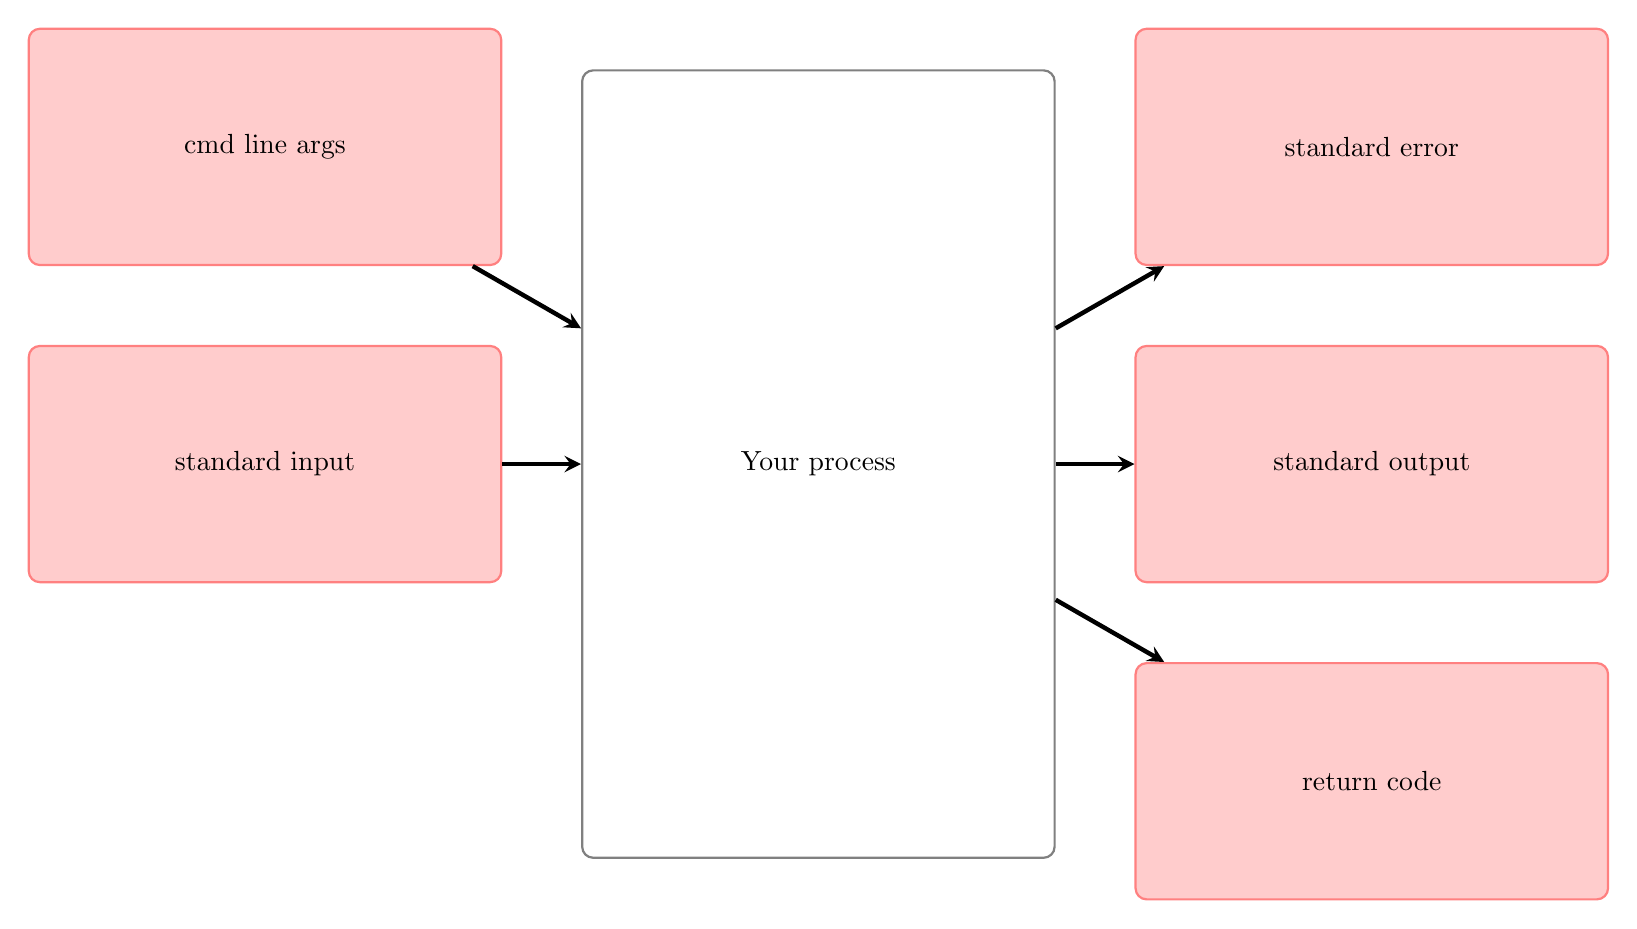
\begin{tikzpicture}
\begin{scope}[node distance=10mm]
	\node (args) [stream] {cmd line args} ;
	\node (stdin) [stream, below =of args] {standard input} ;
	\node (proc)  [myproc, right =of stdin] {Your process} edge [toArrow] (args)  edge [toArrow] (stdin);
	\node (stdout) [stream, right =of proc] {standard output} edge [toArrow] (proc);
	\node (stderr) [stream, above =of stdout] {standard error}  edge [toArrow] (proc) ;
	\node (retcode) [stream, below =of stdout] {return code}  edge [toArrow] (proc) ;
\end{scope}
\end{tikzpicture} 


\myNewSlide
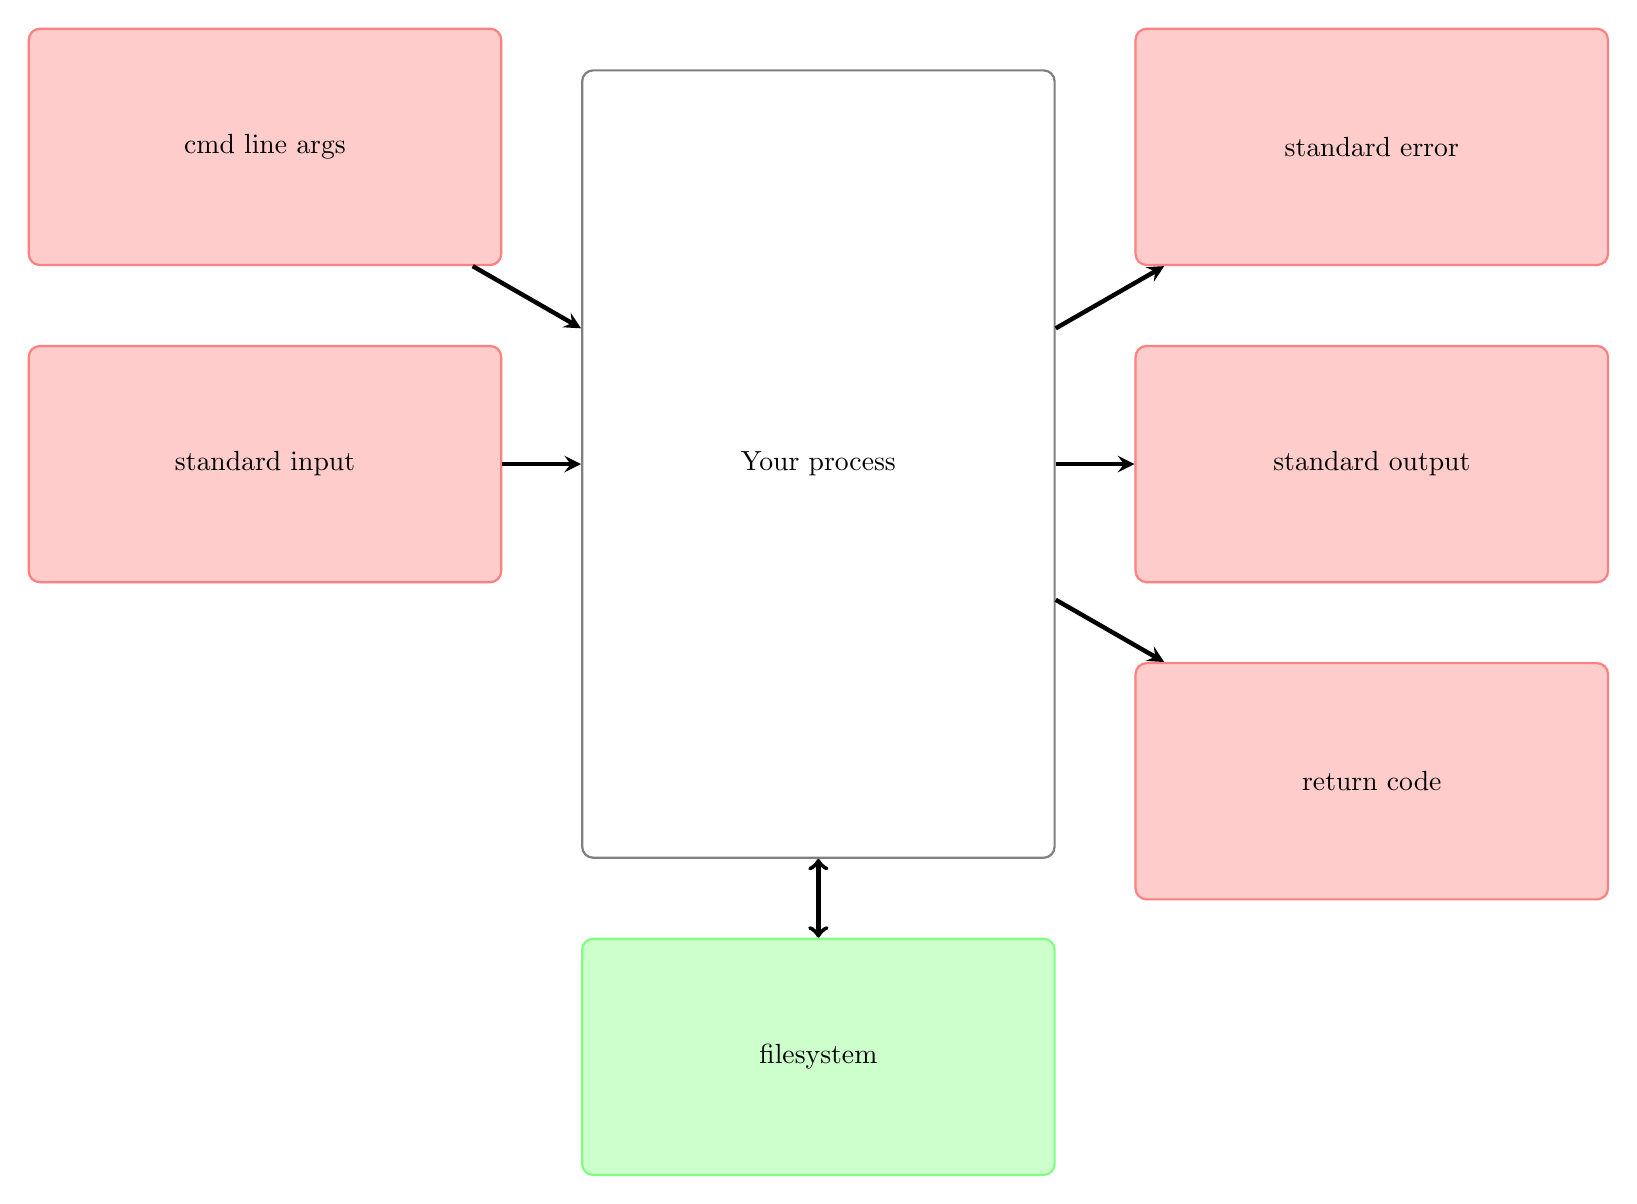
\begin{tikzpicture}
\begin{scope}[node distance=10mm]
	\node (args) [stream] {cmd line args} ;
	\node (stdin) [stream, below =of args] {standard input} ;
	\node (proc)  [myproc, right =of stdin] {Your process} edge [toArrow] (args)  edge [toArrow] (stdin)  ;
	\node (fs) [shared, below =of proc] {filesystem} edge [<->,ultra thick] (proc);
	\node (stdout) [stream, right =of proc] {standard output} edge [toArrow] (proc);
	\node (stderr) [stream, above =of stdout] {standard error}  edge [toArrow] (proc) ;
	\node (retcode) [stream, below =of stdout] {return code}  edge [toArrow] (proc) ;
\end{scope}
\end{tikzpicture} 






\myNewSlide
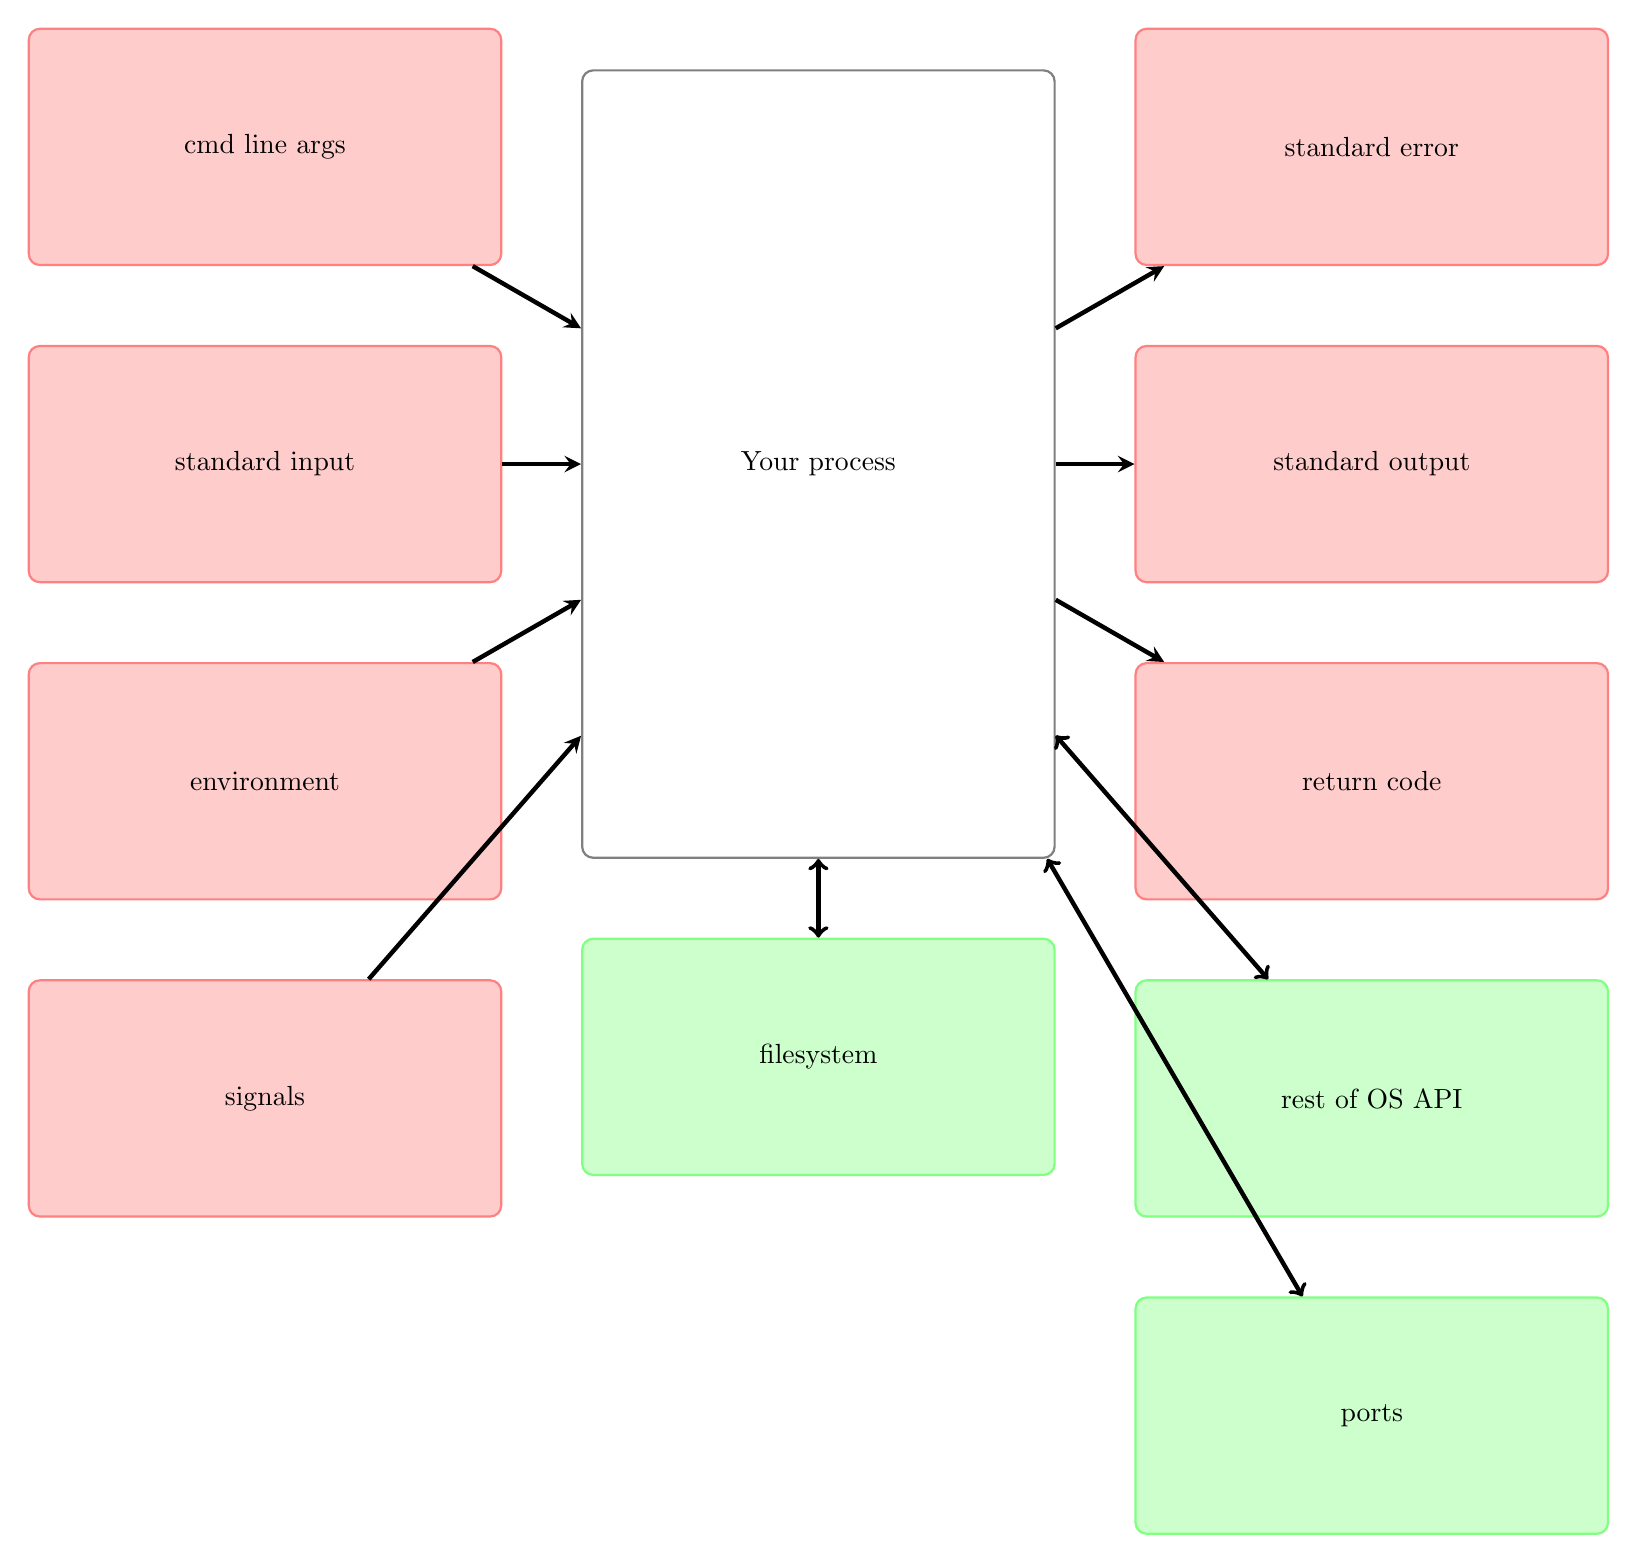
\begin{tikzpicture}
\begin{scope}[node distance=10mm]
	\node (args) [stream] {cmd line args} ;
	\node (stdin) [stream, below =of args] {standard input} ;
	\node (env) [stream, below =of stdin] {environment}  ;
	\node (signals) [stream, below =of env] {signals}  ;
	\node (proc)  [myproc, right =of stdin] {Your process} edge [toArrow] (args)  edge [toArrow] (stdin) edge [toArrow] (env) edge [toArrow] (signals);
	\node (fs) [shared, below =of proc] {filesystem} edge [<->,ultra thick] (proc);
	\node (stdout) [stream, right =of proc] {standard output} edge [toArrow] (proc);
	\node (stderr) [stream, above =of stdout] {standard error}  edge [toArrow] (proc) ;
	\node (retcode) [stream, below =of stdout] {return code}  edge [toArrow] (proc) ;
	\node (sys) [shared, below =of retcode] {rest of OS API} edge [<->,ultra thick] (proc);
	\node (port) [shared, below =of sys] {ports} edge [<->,ultra thick] (proc);
\end{scope}
\end{tikzpicture} 

\myNewSlide
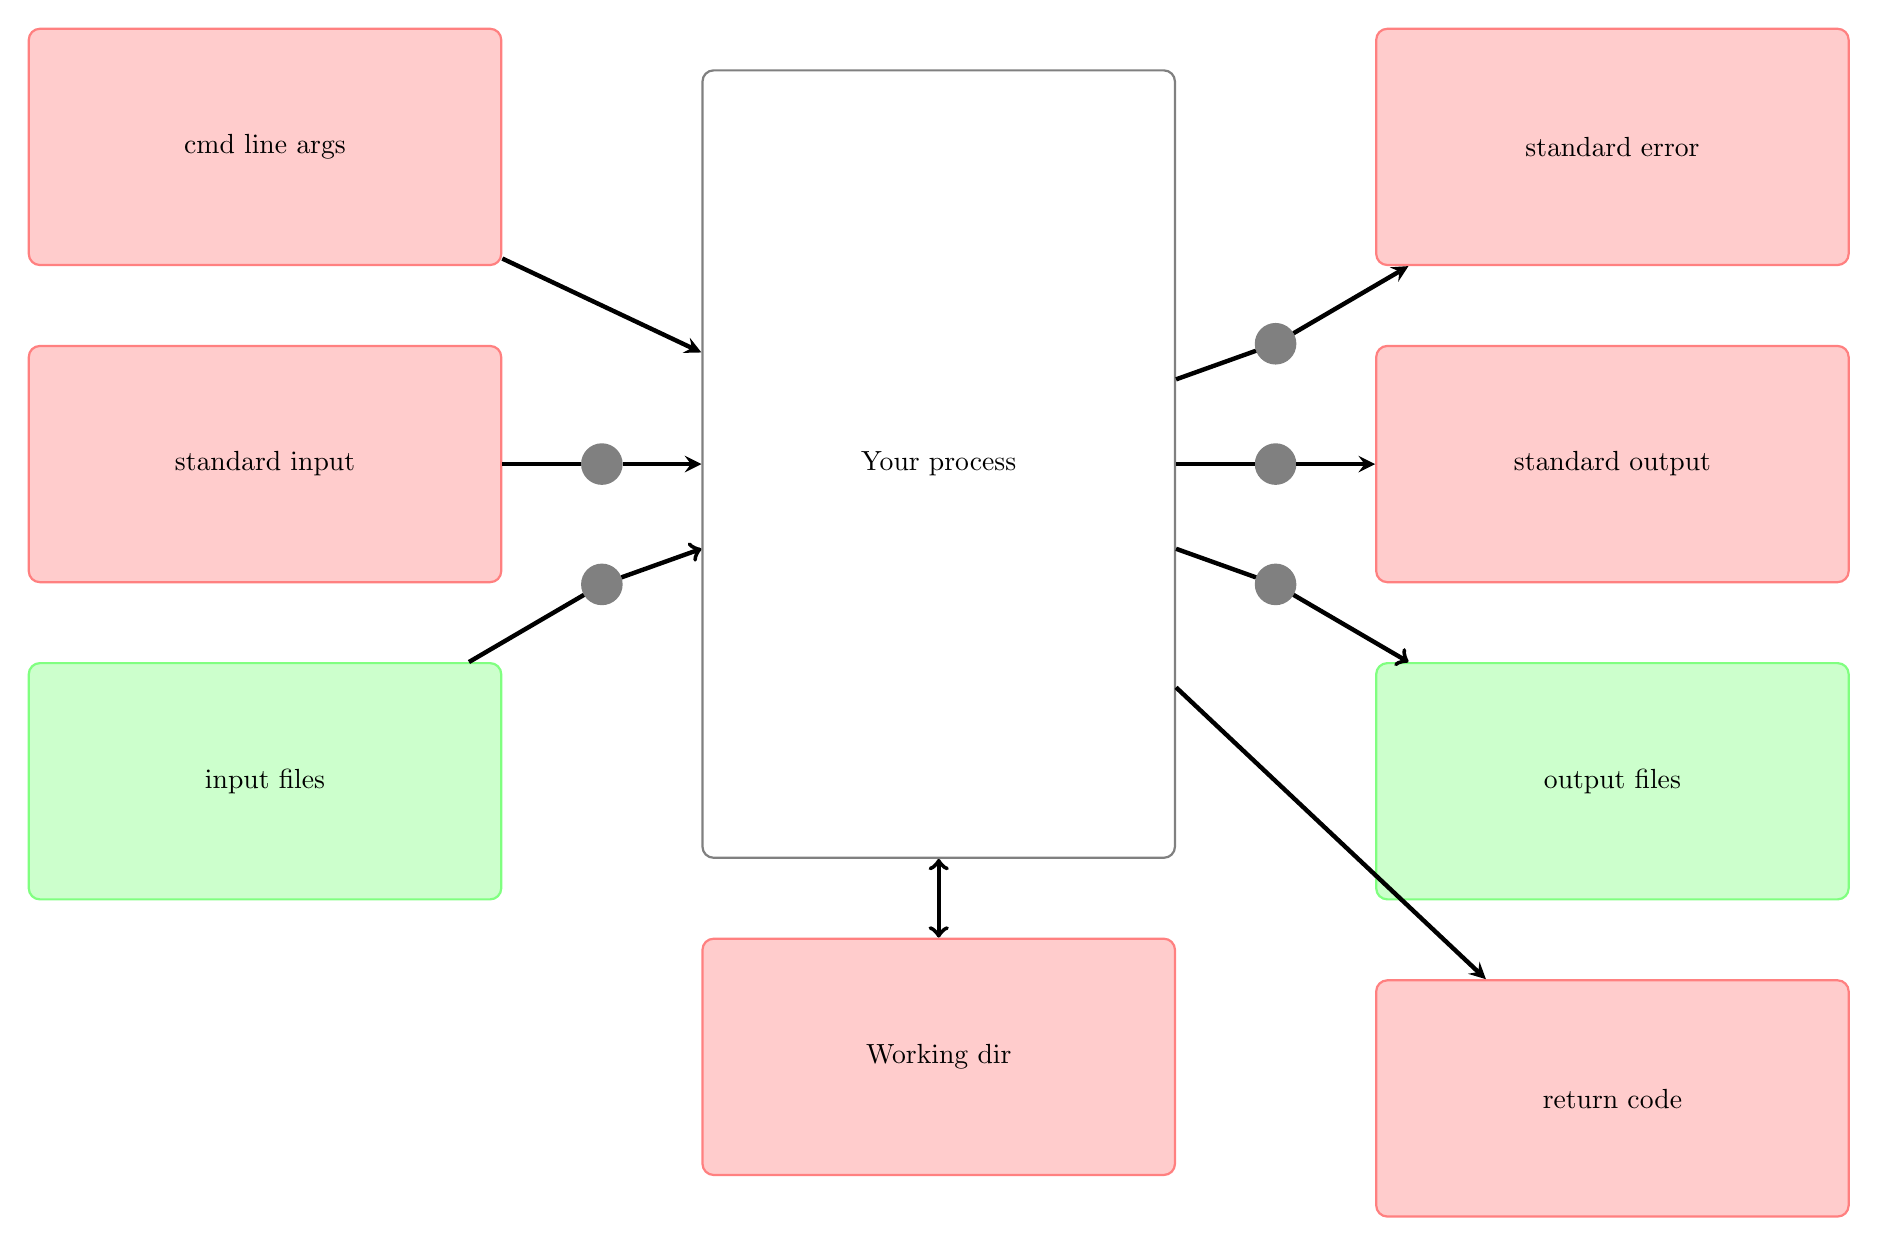
\begin{tikzpicture}
\begin{scope}[node distance=10mm]
	\node (args) [stream] {cmd line args} ;
	\node (stdin) [stream, below =of args] {standard input} ;
	\node (stdinI) [fileI,right = of stdin] {} edge [-,ultra thick] (stdin);
	\node (proc)  [myproc, right =of stdinI] {Your process} edge [toArrow] (args) edge [toArrow] (stdinI);
	 \node (stdoutI) [fileI,right = of proc] {} edge [-,ultra thick] (proc);
	\node (stdout) [stream, right =of stdoutI] {standard output} edge [toArrow] (stdoutI) ;
	 \node (stderrI) [fileI,above = of stdoutI] {} edge [-,ultra thick] (proc);
	\node (stderr) [stream, above =of stdout] {standard error}  edge [toArrow] (stderrI) ;
	 \node (ofsI) [fileI,below = of stdoutI] {} edge [-,ultra thick] (proc);
	\node (ofs) [shared, below =of stdout] {output files} edge [<-,ultra thick] (ofsI);
	 \node (ifsI) [fileI,below = of stdinI] {} edge [->,ultra thick] (proc);
	\node (ifs) [shared, below =of stdin] {input files} edge [-,ultra thick] (ifsI);
	\node (retcode) [stream, below =of ofs] {return code}  edge [toArrow] (proc) ;
	\node (pwd) [stream, below =of proc] {Working dir} edge [<->,ultra thick] (proc);
 edge [->, ultra thick] (proc) ;
\end{scope}
\end{tikzpicture} 


\myNewSlide
\section*{What happened? (more or less)}
\begin{compactitem}
	\item I clicked on the Terminal.app icon in the Dock
	\item Some device driver noted that a click had occurred.
	\item The OS noticed
	\item The OS checked where the cursor was
	\item The OS did some calculations and determined that it was in the ``Dock''
	\item The OS told the \path{Dock} process that a click had occurred.
	\item By asking the OS and doing calculations, the \path{Dock} determined that it was the Terminal.app icon that was clicked.
	\item The \path{Dock} process told the OS to tell the \path{Finder} to launch Terminal.app
	\item \path{Terminal} was launched and {\color{green} it negotiated with the OS and \path{WindowServer} to display a window.}
	\item {\color{green} The \path{Terminal} launched a process called \path{login}}
	\item {\color{black} \path{login} read a history file. Based on this information it wrote a message to its standard output stream. }
	\item {\color{green} \path{Terminal} is reading \path{login}'s output, and \path{Terminal} makes the window display the message.}
	\item {\color{black} \path{login} launched a process called \path{bash}}
	\item {\color{red} \path{bash} initialized itself (by reading files such as\\ \path{/Users/mholder/.bash\_profile})}
	\item {\color{red}\path{bash} wrote its prompt (the characters `$\sim$ 500 \$ ') to its standard error stream.}
	\item {\color{green}\path{Terminal} has wrapped up bash's standard streams (input, output and error stream). When
	it detects that bash wrote something \path{Terminal} does some OS calls to draw the characters in the window.}
	\item {\color{red}\path{bash} told the OS through some function we'll call ``readNextLineOfInput'' that it wanted to read the next line from standard input.  Because there was no input, the execution of the \path{bash}'s process hangs.}
	\item I typed `l'
	\begin{compactenum}	
		\item a keyboard device drive noticed the key was hit and told the OS
		\item the OS asked the window manager what application had ``focus'' -- the answer was \path{Terminal}
		\item The OS told the \path{Terminal} that there was a key-down event
		\item {\color{green}The \path{Terminal} (with help of OS)  the letter `l'}
		\item {\color{green}The \path{Terminal} wrote `l' to a stream that (via OS functions) was connected to \path{bash} standard input}
		\item {\color{green}The \path{Terminal} displayed the letter `l' in the Window}
		\item {\color{red}Because it was not a carriage return, the `readNextLineOfInput' function stored the character, but did not return anything to \path{bash}. So \path{bash} still has not heard anything yet.}
	\end{compactenum}
	\item I typed `s' -- same steps as for when I typed `l'
	\item I typed the `return' key -- steps 1-6 occurred as before.
	\item {\color{red}The `readNextLineOfInput' function that \path{bash} called returned the string `ls$<$newline$>$'}
	\item {\color{red}\path{bash} (through rules we'll talk about later) determined that `ls' means that I wanted to run the program called \path{ls} with no command line arguments.}
	\item Via negotiations with the OS, {\color{red}\path{bash} launched \path{ls}}
	\item Any standard input of \path{bash} will now be redirected to \path{ls}, and the standard output of \path{ls} will be written to the stream, but it will be redirected to \path{bash}'s stdandard output.
	\item \path{ls} checked to see if it got any command line arguments (it did not).
	\item \path{ls} asked the OS what it should use as its working directory (The OS said '/Users/mholder').
	\item \path{ls} asked the OS for the contents of the file '/Users/mholder'
	\item The OS dealt with some filesystem device driver software to get the contents and return the answer.
	\item \path{ls} filtered out any entries in that file that started `.'
	\item \path{ls} queried the OS to find out how many characters wide its standard output was.
	\item \path{ls} formatted the entries such that they fit nicely in the width.
	\item \path{ls} wrote the formatted strings to its standard output.
	\item {\color{red}That standard out from \path{ls} is passed to \path{bash}'s standard output}
	\item {\color{green}\path{Terminal} is reading \path{bash}'s output, and it makes sure that the output is displayed in the window that we see.}
	\item The \path{ls} process is exits
	\item {\color{red}\path{bash} detects that \path{ls} exited. It writes it's prompt again.}
	\item {\color{green}\path{Terminal} displays the latest output from \path{bash}, which is the new prompt.}	
		
\end{compactitem}


\myNewSlide
\path{ls} never deals with \path{bash} (and certainly not with processes further up stream such as \path{login} or \path{Terminal}).
\path{ls} just:
\begin{compactitem}	
	\item checks its command-line arguments,
	\item figures out its working directory (asks the the operating system some context information),
	\item composes an answer to its assigned task,
	\item writes the answer to its standard output stream,
	\item exits
\end{compactitem}

\myNewSlide
\path{bash} never deals with \path{login} or \path{Terminal}.  It just:
\begin{compactenum}	
	\item checks its command-line arguments,
	\item asks the the operating system some context information,
	 \item reads a line of input from standard input,
	\item takes the action requested,
	\item writes ``the answer'' to through its output and error streams,
	\item goes back to step 3
\end{compactenum}

\path{bash} is a shell that is often used to launch other processes. 
So the ``action'' in step 4 is often: ``launch a process and redirect your streams to the new process until it exits.''


\myNewSlide
\section*{Shells}
The interface to the OS and kernel is a huge number of functions -- it easy to invoke these functions in the wrong way, and their ``raw'' response is often cryptic.

Shells:
\begin{compactenum}	
	\item protect the kernel  -- rather than pounding the kernel with our typos, the shell composes valid requests.
	\item make the raw output of system functions human-readable.
\end{compactenum}	

The kernel does not understand text like `ls'

Shells are simple programming language interpreters that take text that humans write, and convert it into instructions for the machine.

\myNewSlide
\normalsize
\begin{compactenum}
	\item The shell is a way of creating a process from the executable and controlling the process' initial context:
	\begin{compactenum}
		\item Specifies command line argument for the process
		\item You can control the environment of the process easily through a shell (we won't tweak the environment much in this course)
		\item The shell's working directory becomes the process's working directory
		\item The shell controls what happens to the process' standard streams (in, out, and err)
		\item The shell captures the return code of the executable as the shell variable '?'
	\end{compactenum}
	\item Failures of commands/executables are denoted by any return code other than 0
	\item \begin{verbatim}>\end{verbatim} will redirect the standard output of a process to a file.
	\item \begin{verbatim}2>\end{verbatim} will redirect the standard error stream of a process to a file.
	\item \begin{verbatim}<\end{verbatim} can be used to redirect a file as standard input
	\item \begin{verbatim}|\end{verbatim} redirects standard output of one process to standard input of another.
\end{compactenum}


\myNewSlide
\normalsize
\path{Bash} line processing:
\begin{algorithmic}[1]
	\STATE Read a line of input (using an OS file-reading function)
	\STATE Tokenize and expand variables
	\STATE The first token is the COMMAND
	\IF{COMMAND is ``exit''}
	\STATE the \path{bash} shell exits
	\ELSIF {COMMAND is a special \path{bash} keyword}
	\STATE take the required action
	\ELSE 
	\STATE {COMMAND should be an executable}
	\IF{An executable called COMMAND is found on \path{bash}'s search path}
		\STATE Launch the executable; give it the other tokens as cmd-line args.
		\STATE Store the return code of the executable in the variable `?'
	\ELSE
		\STATE Give an error message
		\STATE Store 127 in the variable `?'
	\ENDIF
	\ENDIF
	\STATE Go back to step 1
\end{algorithmic}

\myNewSlide
\section*{\path{bash} tokenization and variable expansion}
\begin{compactenum}
	\item tokens are usually delimited by whitespace
	\item to make whitespace a part of a token you have to use quotes or the backslash (escape) mechanism
	\item the \$ in a bash command triggers replacement of the following variable name with the variable's value
	\item single quotes prevent variable substitution
	\item double quotes allow variable substitution
\end{compactenum}


\myNewSlide

\path{Bash} COMMAND  dispatching (How the shell finds executables):
\begin{algorithmic}[1]
	\IF{COMMAND is a path with a directory}
		\IF{the path COMMAND does not exist}
			\STATE print \error{-bash: COMMAND: No such file or directory} and return 127
		\ELSIF {COMMAND is not flagged as an executable}
			\STATE print \error{-bash: COMMAND: Permission denied} and return 126
		\ELSE
			\STATE run the executable COMMAND and return its return code
		\ENDIF
	\ELSE
		\FOR{each DIRECTORY in \path{\$PATH}}
			\IF{the DIRECTORY has an executable called COMMAND}
				\STATE run the executable DIRECTORY/COMMAND and return its return code
			\ENDIF
		\ENDFOR
		\STATE print \error{-bash: COMMAND: command not found} and return 127
	\ENDIF
\end{algorithmic}


\myNewSlide
\section*{Directories and the filesystem}
\begin{compactenum}
	\item hierarchical (like a phylogenetic classification where the higher level groups correspond to directories)
	\item directories are separated by \path{/}
	\item you can specify paths by:
		\begin{compactenum}
			\item their absolute location (always starts with \path{/} for the root of the file system), or
			\item the path relative to the current working directory.
		\end{compactenum}
	\item The current directory is denoted with a dot \path{.} 
	\item The parent directory is denoted with a two dots \path{..} 
	\item The grandparent directory is :\path{../..} 
	\item These rules for finding file paths apply to the OS library calls for opening files as well as \path{bash} (In python we'll see the same rules).
	\item filename that start with a dot are ``hidden''
\end{compactenum}

\myNewSlide
\textwidth 10in
\oddsidemargin -0.7in

\normalsize
\begin{table}[htdp]
\begin{center} \normalsize
\begin{tabular}{|c|p{18cm}}
\hline
\path{ls} & list the contents of a directory \\
 &  \example{ls -l .Trash}\\
\hline
\path{echo} & writes the command line arguments (separating them with a space) to standard error\\
 & \example{echo hi there}\\
\hline
\path{cd} & change the shell's working directory
\\ & \example{cd Desktop}\\
\hline
\path{mkdir} & create a new directory\\ & \example{mkdir tmp}\\
\hline
\path{rm} & Remove a file (or directory if the \example{-r} is used). {\color{red} Be Careful!! -- their is no UNDO !}\\ & \example{rm a.out}\\
\hline
\path{cp} & Copy a file (or directory if the \path{-r} is used)  to a new location\\ & \example{cp src dest}\\
\hline
\end{tabular}
\end{center}
\label{default}
\end{table}%


\myNewSlide
\begin{table}[htdp]
\begin{center}
\begin{tabular}{|c|p{18cm}}
\hline
\path{mv} & Move a file (or directory if the \path{-r} is used)  to a new location\\ & \example{mv orig new}\\
\hline
\path{man} & Uses the PAGER interface to look at a help page for a command (it may be easier to use google to find the man page)\\ & \example{man rm}\\
\hline
\path{pwd} & writes the path to the current working directory to standard out\\ & \example{pwd}\\
\hline
\path{env} & writes all of the shell variables to standard out\\ & \example{env}\\
\hline
\path{ssh} & starts a \path{login} on another machine\\ & \example{ssh phylo.bio.ku.edu}\\
\hline
\path{scp} & like \path{cp} but can copy to a remote machine\\ & \example{scp src 129.237.138.127:dest}\\
\hline
\end{tabular}
\end{center}
\label{default}
\end{table}%

\myNewSlide
\begin{table}[htdp]
\begin{center}
\begin{tabular}{|c|p{18cm}}
\hline
\path{cat, tail, head} & Write contents of a file to standard out\\ & \example{cat x.txt}\\
\hline
\path{wc} & Counts words, characters, or lines in a file\\ & \example{wc -l x.txt}\\
\hline
\path{which} & Writes the full path to an executable to standard out\\ & \example{which ls}\\
\hline
\path{ps} & Lists the running processes\\ & \example{ps auxww}\\
\hline
\path{chmod} & Change the mode of a file. This is how we grant read/write/executable permissions.\\ & \example{chmod +x echo.py} would make \path{echo.py} executable\\
\hline
\end{tabular}
\end{center}
\label{default}
\end{table}%


\myNewSlide
\textwidth 8in
\oddsidemargin -0.0in

\section*{Efficiency tricks}
\normalsize
\begin{compactenum}
	\item arrow up and arrow down to move through your command history
	\item \path{Control-a} moves the cursor to the front of a line; \path{Control-e} to the end.
	\item \path{Meta-f} moves the cursor forward one word; \path{Meta-b} move back one word.
	\item \example{history} displays your history. The command \example{!34} would repeat the 34th command.
	\item Hitting the \path{Tab}-key when you are typing in \path{bash} will autocomplete paths
	\item \example{cd -} takes you back to your previous working directory.
	\item use a \example{alias shortname='long command here'} in your home directory's \path{.bash\_profile} file to make shortcuts to commonly used, but cumbersome commands (one to open a file in your preferred text editor is nice).
	\item On Mac, \example{open filename} opens the path `filename' in whatever the Finder thinks is the appropriate application.
\end{compactenum}


\myNewSlide
\large
{\bf Software} -- instructions for a computer.\\
{\bf A program} -- text that conforms to the definition of a programming language. The program is not written in the binary operations that the hardware can operate on.  It has to be translated into the language of the machine.\\
{\bf Compiled languages:}\\
1. {\color{red} Your program} $\rightarrow$ (compiler) $\rightarrow$ executable\par
Then you have to launch the executable:\\
2. executable $\rightarrow$ (kernel) $\rightarrow$ running process $\rightarrow$ {\color{red} Your results}\\
{\bf Interpreted languages:}\\
1. interpreter executable $\rightarrow$ (kernel) $\rightarrow$ running interpreter process\\
2. {\color{red} Your script}  $\rightarrow$ (interpreter process) $\rightarrow$ {\color{red} Your results}

\myNewSlide
\section*{Python}
\begin{compactenum}
	\item an interpreted procedural language with good support for lots of programming tasks
	\item free
	\item terse, but clear syntax
	\item platform-independent (and your python programs will be if you don't do weird things)
	\item execution speed is slow (but that rarely matters)
	\item mature and stable (lots of libraries, runs reliably on any modern computer)
	\item Comes with standard \path{sys}, \path{os}, and \path{subprocess} libraries for interacting with the Operating System.
\end{compactenum}

\myNewSlide
\section*{Memory}
\large
\begin{compactenum}
	\item internally all memory is binary -- bytes on the hard disk
	\item a semantic (interpretation) step is needed to express complex data
\end{compactenum}

\end{document}
